\documentclass{article}

\usepackage{sbc-template}
\usepackage[brazil]{babel}
\usepackage[utf8]{inputenc}
\usepackage{color}
\usepackage[table,xcdraw]{xcolor}
\usepackage{float}
\usepackage{graphicx,url}
\usepackage{hyperref}
\usepackage{hypcap}
\usepackage{longtable}
\usepackage{microtype}
\usepackage{multirow}
\usepackage{pgfplots, pgfplotstable}
\usepackage[brazilian,hyperpageref]{backref}     % Paginas com as citações na bibl
\usepackage[alf]{abntex2cite}   % Citações padrão ABNT
\usepackage{indentfirst}
\usepackage{filecontents}
\usetikzlibrary{patterns}
% ---
% Configurações do pacote backref
% Usado sem a opção hyperpageref de backref
\renewcommand{\backrefpagesname}{Citado na(s) página(s):~}
% Texto padrão antes do número das páginas
\renewcommand{\backref}{}
% Define os textos da citação
\renewcommand*{\backrefalt}[4]{
    \ifcase #1 %
        Nenhuma citação no texto.%
    \or
        Citado na página #2.%
    \else
        Citado #1 vezes nas páginas #2.%
    \fi}%
% ---
\makeatletter
\hypersetup{
  pdftex,
  pdftitle={\@title}, 
  pdfauthor={\@author},
  pdfsubject={Artigo Científico},
  pdfcreator={LaTeX with sublime text},
  pdfkeywords={aprendizado de máquina}{artigo científico}{redações}{enem}, 
  colorlinks=true,   % false: boxed links; true: colored links
  linkcolor=blue,    % color of internal links
  citecolor=blue,    % color of links to bibliography
  filecolor=magenta, % color of file links
  urlcolor=blue,
  bookmarksdepth=4
}
\makeatother

% Seleciona o idioma do documento (conforme pacotes do babel)
\selectlanguage{brazil}

% \setlength{\textfloatsep}{5pt}
% \setlength{\parindent}{0pt}
% \setlength{\intextsep}{10pt}

\sloppy

\title{Recuperação de Padrões na Valoração Textual de Redações}

\author{Eugênio Cunha\inst{1}, Marco Túlio Alves Nolasco Rodrigues\inst{1}}

\address{Universidade de Itaúna (UIT)\\
  Caixa Postal 100 -- 35.680-142 -- Itaúna -- MG -- Brasil
  \email{\{genio.py, tulio.rodrigues\}@gmail.com}
}

\begin{document} 

\maketitle
    
\begin{abstract}
  Nowadays, there is an intense amount of essays being produced and evaluated 
  in entrance exams, competitions and exams. Unlike the manuals, which process 
  and evaluate the essays manually, this work addresses an automatic way, 
  through machine learning, capable of generalizing, learning and extracting 
  standards from writing based on the labeled content. The method needs little 
  human intervention and allows the valuation of large amounts of texts. This 
  job is based on the problem of manual assessment of competences required in a 
  essay-argumentative writing text with diverse themes social, scientific, 
  cultural or political. Given a corpus of the main objective is to induce a 
  model to classify the required by writing an evaluation note on the text. 
  Embasado in the main metrics of analysis of the classifiers cited in the 
  literature of machine learning, the solution proposed in this work was shown 
  to be useful and useful for use in issues involving text valuation manual by 
  trained professionals.
\end{abstract}
\begin{resumo} 
  Nos dias atuais, há uma quantidade intensa de redações sendo produzida e 
  avaliada em vestibulares, concursos e exames. Diferentemente dos métodos 
  existentes, que processam e avaliam as redações de maneira manual, este 
  trabalho aborda uma forma automática, por meio de  aprendizagem de máquina, 
  capaz de generalizar, aprender e extrair padrões das classes de redações com 
  base no conteúdo rotulado. O método precisa de pouca intervenção humana e 
  permite a valoração de grandes quantidades de textos.  Este trabalho 
  fundamenta-se no problema de avaliação manual das competências exigidas em um 
  texto de redação do tipo dissertativo-argumentativo com temas diversificados 
  de ordem social, científica, cultural ou política. Dado um ``corpus'' de 
  redações o objetivo principal é induzir um modelo a classificar as 
  competências exigidas compondo uma nota avaliativa sobre o texto. Embasado 
  nas principais métricas de análise dos classificadores citados na literatura 
  de aprendizado de máquina, a solução proposta neste trabalho demonstrou ser 
  útil e propícia a ser utilizada em problemas que envolva a valoração de texto 
  manual por profissionais capacitados.
\end{resumo}

\newpage
\section{Introdução}

O desenvolvimento de uma redação é uma atividade prática, presente na 
cultura civilizada desde a invenção da escrita. \citeonline{lara:1995}, 
explica em seu trabalho, que com o fim da ditadura iniciou-se processo de 
redemocratização, que consequentemente, restitui a palavra ao estudante. 
O decreto 79 298, de 24 de fevereiro de 1977, definiu a volta da redação à 
escola, pela ``inclusão obrigatória da prova ou questão de redação em língua 
portuguesa'' nos concursos e vestibulares (Art. 1º, alínea d). A prova de 
redação tem sido utilizada de forma ampla em concursos, vestibulares e exames, 
tal como o ENEM, hoje o maior exame do Brasil, que no ano de 2016, contou com 
8 627 195 inscrições e a participação direta de 11 360 profissionais externos, 
na correção de 5 825 134 redações, segundo o relatório de gestão 
\citeauthor{relatorio_de_gestao:2016} (\citeyear{relatorio_de_gestao:2016}). 
Com o advento do ENEM ser um requisito para o processo seletivo de acesso às 
inúmeras universidades públicas ~\cite{sisu:2017} e a importantes programas de 
governo ~\cite{csf:2017}, este número tem aumentado, incessantemente.

Com o processamento computacional mais barato e poderoso, a crescente variedade 
e volume de dados disponíveis e o armazenamento de forma acessível, o 
Aprendizado de Máquina está no centro de muitos avanços tecnológicos, 
alcançando as áreas, antes exclusivas de seres humanos. Os carros autônomos do
projeto \citeonline{waymo:2017}, são o exemplo de uma atividade, antes 
exclusivamente humana, hoje exercida e aperfeiçoada por algoritmos de 
Aprendizado de Máquina. 

A avaliação automática de redações pode ser realizada utilizando sistemas
especialistas ou algoritmos de Aprendizado de Máquina. A primeira hipótese, 
dependente essencialmente da presença de especialistas, que detêm o 
conhecimento sobre o domínio do problema para desenvolver um conjunto de 
regras. \citeonline{negnevitsky2005artificial}, explica que o sistema 
especialista deve ser capaz de tomar suas decisões, ou seja, as regras são 
disparadas para atingir determinadas opções. Entretanto, regras desenvolvidas 
manualmente, tem um processo de manutenção e atualização complexo, o que torna 
difícil a sua utilização em diferentes domínios do problema proposto. O uso de 
algoritmos de Aprendizado de Máquina, na valoração de redações, é uma 
alternativa ao sistema especialista, exige menor esforço humano, com a simples 
abstração de extrair padrões ou características, aprender e generalizar. 

Devido à grande quantidade de redações produzidas em concursos, vestibulares 
e exames, torna-se humanamente difícil e caro, organizar e avaliar as 
competências de uma redação manualmente. A hipótese deste artigo é que um 
algoritmo de Aprendizado de Máquina pode ser útil e propício, quando utilizado 
em problemas que envolva a valoração de textos. Para avaliar e validar a 
hipótese, o método de construção do conhecimento deste estudo terá como 
fundamento o problema da recuperação de padrões, na valoração textual. Dado 
dois classificadores, com lógicas de classificação distintas, induzir ambos, a 
recuperar padrões implicitos num \textit{corpus} de redações e classificar a 
competência exigida num texto de redação em uma nova amostra, automaticamente.

Além disso, o presente estudo, com base na proposta do problema descrito, 
contribuirá na área do Aprendizado de Máquina e diretamente no processo de 
valoração de um texto em prosa do tipo dissertativo-argumentativo.
\section{Trabalhos Relacionados}


Este tópico é destinado a listar uma sequência de trabalhos científicos nas 
áreas abordadas por este estudo com o objetivo de adquirir conhecimento para a
elaboração do mesmo.

De acordo com \cite{silvio_taynan:2017}, à prova de redação do ENEM é avaliada 
levando em conta uma matriz de referência listada na Tabela 
\ref{table:matriz_referencia}. Essa matriz, desenvolvida pelo 
\cite{edital_enem:2016}, com a colaboração de especialistas, foi elaborada com 
o objetivo de operacionalizar o exame. A matriz apresenta cinco competências, 
para cada competência expressa para redação existem níveis de conhecimento 
associados de 0 a 5.

\begin{longtable}{|c|l|l|}
    \caption{Competência I de V da matriz de referência elaborada pelo
    \cite{matriz_referencia_redacao:2016}.}
    \label{table:matriz_referencia}
    \endfirsthead
    \hline
    \multirow{7}{*}{\textbf{I}} & \multicolumn{2}{l|}{\textbf{Demonstrar domínio da norma padrão da língua escrita.}} \\ \cline{2-3} 
     & 0 & \begin{tabular}[c]{@{}l@{}}Demonstra desconhecimento da modalidade escrita formal da \\ língua portuguesa.\end{tabular} \\ \cline{2-3} 
     & 1 & \begin{tabular}[c]{@{}l@{}}Demonstra domínio precário da modalidade escrita formal da \\ língua portuguesa, de forma sistemática, com diversificados e \\ frequentes desvios gramaticais, de escolha de registro e de \\ convenções da escrita.\end{tabular} \\ \cline{2-3} 
     & 2 & \begin{tabular}[c]{@{}l@{}}Demonstra domínio insuficiente da modalidade escrita formal \\ da língua portuguesa, com muitos desvios gramaticais, de \\ escolha de registro e de convenções da escrita.\end{tabular} \\ \cline{2-3} 
     & 3 & \begin{tabular}[c]{@{}l@{}}Demonstra domínio mediano da modalidade escrita formal da \\ língua portuguesa e de escolha de registro, com alguns desvios \\ gramaticais e de convenções da escrita.\end{tabular} \\ \cline{2-3} 
     & 4 & \begin{tabular}[c]{@{}l@{}}Demonstra bom domínio da modalidade escrita formal da língua \\ portuguesa e de escolha de registro,com poucos desvios \\ gramaticais e de convenções da escrita.\end{tabular} \\ \cline{2-3} 
     & 5 & \begin{tabular}[c]{@{}l@{}}Demonstra excelente domínio da modalidade escrita formal da \\ língua portuguesa e de escolha de registro. Desvios gramaticais \\ ou de convenções da escrita serão aceitos somente como \\ excepcionalidade e quando não caracterizem reincidência.\end{tabular} \\ \hline
    % \multirow{7}{*}{\textbf{II}} & \multicolumn{2}{l|}{\textbf{\begin{tabular}[c]{@{}l@{}}Compreender a proposta de redação e aplicar conceitos \\ das varias áreas de conhecimento para desenvolver o tema, \\ dentro dos limites estruturais do texto \\ dissertativo-argumentativo em prosa.\end{tabular}}} \\ \cline{2-3} 
    %  & 0 & \begin{tabular}[c]{@{}l@{}}``Fuga ao tema/não atendimento à estrutura \\ dissertativo-argumentativa''.\end{tabular} \\ \cline{2-3} 
    %  & 1 & \begin{tabular}[c]{@{}l@{}}Apresenta o assunto, tangenciando o tema ou demonstra \\ domínio precário do texto dissertativo-argumentativo, com \\ traços constantes de outros tipos textuais\end{tabular} \\ \cline{2-3} 
    %  & 2 & \begin{tabular}[c]{@{}l@{}}Desenvolve o tema recorrendo à cópia de trechos dos textos \\ motivadores ou apresenta domínio insuficiente do texto \\ dissertativo-argumentativo, não atendendo à estrutura com \\ proposição, argumentação e conclusão.\end{tabular} \\ \cline{2-3} 
    %  & 3 & \begin{tabular}[c]{@{}l@{}}Desenvolve o tema por meio de argumentação previsível e \\ apresenta domínio mediano do texto dissertativo-argumentativo, \\ com proposição, argumentação e conclusão.\end{tabular} \\ \cline{2-3} 
    %  & 4 & \begin{tabular}[c]{@{}l@{}}Desenvolve o tema por meio de argumentação consistente e \\ apresenta bom domínio do texto dissertativo-argumentativo, \\ com proposição, argumentação e conclusão.\end{tabular} \\ \cline{2-3} 
    %  & 5 & \begin{tabular}[c]{@{}l@{}}Desenvolve o tema por meio de argumentação consistente, a \\ partir de um repertório sócio cultural produtivo e apresenta \\ excelente domínio do texto dissertativo-argumentativo.\end{tabular} \\ \hline
    % \multirow{7}{*}{\textbf{III}} & \multicolumn{2}{l|}{\textbf{\begin{tabular}[c]{@{}l@{}}Selecionar, relacionar, organizar e interpretar informações, \\ fatos, opiniões e argumentos em defesa de um ponto de vista.\end{tabular}}} \\ \cline{2-3} 
    %  & 0 & \begin{tabular}[c]{@{}l@{}}Apresenta informações, fatos e opiniões não relacionados \\ ao tema e sem defesa de um ponto de vista.\end{tabular} \\ \cline{2-3} 
    %  & 1 & \begin{tabular}[c]{@{}l@{}}Apresenta informações, fatos e opiniões pouco relacionados \\ ao tema ou incoerentes e sem defesa de um ponto de vista.\end{tabular} \\ \cline{2-3} 
    %  & 2 & \begin{tabular}[c]{@{}l@{}}Apresenta informações, fatos e opiniões relacionados ao \\ tema, mas desorganizados ou contraditórios e limitados aos \\ argumentos dos textos motivadores, em defesa de um \\ ponto de vista.\end{tabular} \\ \cline{2-3} 
    %  & 3 & \begin{tabular}[c]{@{}l@{}}Apresenta informações, fatos e opiniões relacionados ao tema, \\ limitados aos argumentos dos textos motivadores e pouco \\ organizados, em defesa de um ponto de vista.\end{tabular} \\ \cline{2-3} 
    %  & 4 & \begin{tabular}[c]{@{}l@{}}Apresenta informações, fatos e opiniões relacionados ao tema, \\ de forma organizada, com indícios de autoria, em defesa de \\ um ponto de vista.\end{tabular} \\ \cline{2-3} 
    %  & 5 & \begin{tabular}[c]{@{}l@{}}Apresenta informações, fatos e opiniões relacionados ao \\ tema proposto, de forma consistente e organizada, configurando \\ autoria, em defesa de um ponto de vista.\end{tabular} \\ \hline
    % \multirow{7}{*}{\textbf{IV}} & \multicolumn{2}{l|}{\textbf{\begin{tabular}[c]{@{}l@{}}Demonstrar conhecimento dos mecanismos linguísticos \\ necessários para a construção da argumentação.\end{tabular}}} \\ \cline{2-3} 
    %  & 0 & Não articula as informações. \\ \cline{2-3} 
    %  & 1 & Articula as partes do texto de forma precária. \\ \cline{2-3} 
    %  & 2 & \begin{tabular}[c]{@{}l@{}}Articula as partes do texto, de forma insuficiente, com muitas \\ inadequações e apresenta repertório limitado de recursos coesivos.\end{tabular} \\ \cline{2-3} 
    %  & 3 & \begin{tabular}[c]{@{}l@{}}Articula as partes do texto, de forma mediana, com inadequações, \\ e apresenta repertório pouco diversificado de recursos coesivos.\end{tabular} \\ \cline{2-3} 
    %  & 4 & \begin{tabular}[c]{@{}l@{}}Articula as partes do texto com poucas inadequações e apresenta \\ repertório diversificado de recursos coesivos.\end{tabular} \\ \cline{2-3} 
    %  & 5 & \begin{tabular}[c]{@{}l@{}}Articula bem as partes do texto e apresenta repertório diversificado \\ de recursos coesivos.\end{tabular} \\ \hline
    % \multirow{7}{*}{\textbf{V}} & \multicolumn{2}{l|}{\textbf{\begin{tabular}[c]{@{}l@{}}Elaborar proposta de intervenção para o problema abordado, \\ respeitando os direitos humanos.\end{tabular}}} \\ \cline{2-3} 
    %  & 0 & \begin{tabular}[c]{@{}l@{}}Não apresenta proposta de intervenção ou apresenta proposta não \\ relacionada ao tema ou ao assunto.\end{tabular} \\ \cline{2-3} 
    %  & 1 & \begin{tabular}[c]{@{}l@{}}Apresenta proposta de intervenção vaga, precária ou relacionada \\ apenas ao assunto.\end{tabular} \\ \cline{2-3} 
    %  & 2 & \begin{tabular}[c]{@{}l@{}}Elabora, de forma insuficiente, proposta de intervenção relacionada \\ ao tema, ou não articulada com adiscussão desenvolvida no texto.\end{tabular} \\ \cline{2-3} 
    %  & 3 & \begin{tabular}[c]{@{}l@{}}Elabora, de forma mediana, proposta de intervenção relacionada ao \\ tema e articulada à discussão desenvolvida no texto.\end{tabular} \\ \cline{2-3} 
    %  & 4 & \begin{tabular}[c]{@{}l@{}}Elabora bem proposta de intervenção relacionada ao tema e \\ articulada à discussão desenvolvida no texto.\end{tabular} \\ \cline{2-3} 
    %  & 5 & \begin{tabular}[c]{@{}l@{}}Elabora muito bem proposta de intervenção, detalhada, relacionada \\ ao tema e articulada à discussão desenvolvida no texto.\end{tabular} \\ \hline
\end{longtable}

De acordo com \cite{braga:2015}, no texto de redação, o candidato defenderá 
uma opinião a respeito do tema proposto, de forma coerente e coesa, embasado em 
argumentos consistentes. O texto será redigido respeitando a escrita formal da 
Língua Portuguesa. Ao fim, o candidato elabora uma proposta de intervenção 
social para o problema apresentado no desenvolvimento do texto que respeite os 
direitos humanos.

Segundo \cite{monard_baranauskas:2003} ``A indução é a forma de inferência 
lógica que permite obter conclusões genéricas sobre um conjunto particular de 
exemplos.'' Na indução, um conceito é aprendido efetuando-se inferência 
indutiva sobre os exemplos apresentados. O aprendizado indutivo pode ser 
dividido em supervisionado e não-supervisionado como ilustrada a Figura 
\ref{figure:aprendizado_indutivo}. No aprendizado não-supervisionado, o 
algoritmo de aprendizado analisa os exemplos fornecidos e tenta determinar se 
alguns deles podem ser agrupados de alguma maneira, formando \textit{clusters} 
ou agrupamentos. Já no aprendizado supervisionado é fornecido ao algoritmo de 
aprendizado um conjunto de exemplos de treinamento para os quais o rótulo da 
classe associada é conhecido.

\begin{figure}[H]
\begin{center}
    
\includegraphics[scale=0.40]{images/aprendizado_indutivo.png}
\end{center}
\caption{Árvore hierárquica do aprendizado indutivo, a qual é dividida em 
algoritmos supervisionado e não-supervisionado.}
\label{figure:aprendizado_indutivo}
\end{figure}

De acordo com \cite{porthos_motta:2016}, classificadores são utilizados para a 
predição de classes de objetos e pode ser dita como o processo de generalização 
dos dados a partir de diferentes instâncias. Existe uma tendência de se referir 
a problemas com uma resposta quantitativas como problemas de regressão e 
aqueles com uma resposta qualitativa como problemas de classificação. Dado um 
conjunto de exemplos como ilustrado na Figura 
\ref{figure:processo_classificacao}, os classificadores devem encontrar uma 
função geral capaz de prever adequadamente as saídas para novos exemplos, após 
o treinamento, o classificador é avaliado e se necessário o processo de 
classificação pode ser ajustado usando o conhecimento sobre o domínio do 
problema para escolher os dados de entrada ao algoritmo de aprendizado.

\begin{figure}[H]
\begin{center}
    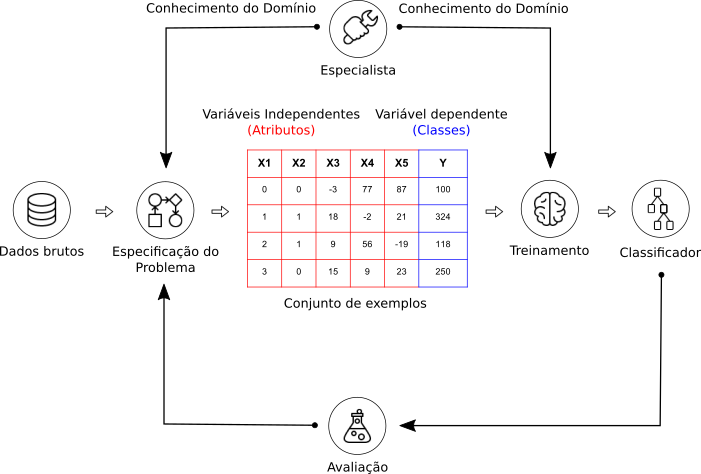
\includegraphics[scale=0.60]{images/processo_classificacao.png}
\end{center}
\caption{Fluxo do processo de classificação, o modelo encontra uma função geral 
capaz de prever as saídas, a especificação do problema pode ser reajustada com 
o conhecimento do domínio para obter um melhor resultado.}
\label{figure:processo_classificacao}
\end{figure}

Diversas ferramentas disponíveis para exploração de dados dispõem de soluções 
para o processamento e a análise das informações de forma ágil e simples. 
Em uma análise comparativa \cite{boscarioli2014avaliaccao} demonstra que não 
existe uma única ferramenta com características melhores para todas as 
aplicações em mineração de dados. Em um estudo que comparou quatro ferramentas 
(KMINE, \textit{Orange}, Tanagra, Weka), todas de código aberto, gratuitas e 
muito utilizadas na pesquisa e na academia, \cite{wahbeh2011comparison} 
concluiu que a ferramenta Weka apresentou o melhor desempenho, seguido pelo 
\textit{Orange}, e, depois, pelo KMINE e Tanagra. De acordo com 
\cite{JMLR:demsar13a}, a ferramenta \textit{Orange} na atual versão 3.5 
desenvolvida pelo laboratório de Inteligência Artificial da Faculdade de 
Computação e Ciência da Informação da Universidade de \textit{Ljubljana} na 
\textit{Eslovênia} sob a licença GPL, possui uma interface gráfica denominada 
\textit{Orange Canvas}. Por meio de sua interface ilustrada na Figura 
\ref{figure:orange_canvas} é possível conectar e interligar os objetos 
montando um fluxo de trabalho para o desenvolvimento de modelos de 
classificação, incluindo \textit{Adaboost}, \textit{Naive Bayes}, Regras de 
Decisão, Árvores de Decisão, etc..

\begin{figure}[H]
\begin{center}
    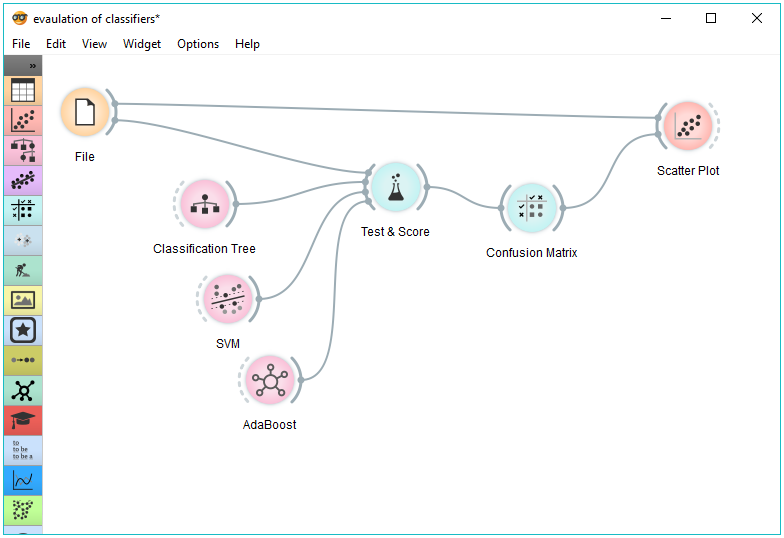
\includegraphics[scale=0.50]{images/orange_canvas.png}
\end{center}
\caption{Ferramenta de mineração de dados \textit{Orange Canvas}} 
executando teste de desempenho dos classificadores AdaBoost, SVM e 
\textit{Classification Tree} na matriz de confusão.  
\label{figure:orange_canvas}
\end{figure}

No processo de mineração de dados, segundo \cite{matsubara2003pretext}, na 
etapa de pré-processamento de textos, um dos métodos geralmente adotado é a 
representação usando a abordagem ``bag-of-words'', uma das representações 
estruturadas mais simples, que utiliza técnicas de redução do termo ao seu 
radical e remoção de termos irrelevantes. Cada documento é  representado como 
um vetor de palavras que ocorrem no documento, especificamente uma tabela 
atributo-valor. 

Segundo o estudo de \cite{de2017mineraccao}, o classificador Naive Bayes é um 
progenitor probalístico para textos, está entre um dos mais utilizados no 
Aprendizado de Máquina, devido a seu comportamento simplista que traz bons 
resultados em muitos casos. Baseado no Teorema de Bayes, criado por Thomas 
Bayes no século XVIII, este classificador é eleito o mais eficiente na precisão 
e rotulação de novas amostras \cite{chakrabarti2002mining}. Objetivo da 
classificação Naive Bayes é encontrar a melhor classe, uma característica 
atraente desse classificador.

Um dos algoritmos mais famoso e utilizado no Aprendizado de Máquina é 
\textit{AdaBoost} ou \textit{Adaptive Boosting} derivado do \textit{Boosting}, 
uma técnica de Aprendizado de Máquina que usa diversos classificadores 
fracos com a finalidade de aumentar a acurácia geral. Segundo 
\cite{dos2015detecccao}, o seu sucesso deve-se ao merito de conseguir 
adaptar-se aos classificadores base. Neste algoritmo, classificadores são 
gerados de forma a favorecer os exemplos erroneamente classificados pelos
classificadores anteriores.


% Baseado em Boosting

% Boosting é uma técnica de aprendizado de máquina que combina diversos classificadores fracos com o objetivo de melhorar a acurácia geral. Em
% cada iteração, o algoritmo atualiza os pesos dos exemplos e constrói um
% classificador adicional. Um esquema simples de votação é utilizado para
% combinar os classificadores. O algoritmo mais famoso baseado em Boosting
% é o AdaBoost. Este algoritmo aumenta os pesos dos exemplos em que os
% classificadores anteriores cometeram erros. Assim, foca o classificador adi-
% cional nos exemplos mais difı́ceis. Inicialmente, uma distribuição uniforme
% de pesos é atribuı́da aos exemplos.

% Adaboost

% O emprego de técnicas de mineração de textos pode auxiliar no mapeamento de
% documentos. Neste escopo, o uso de abordagens de mineração de texto para
% classificação de documentos é de grande interesse. Uma categoria de algoritmos de
% aprendizado de máquina que tem sido usada com sucesso para classificação de
% documentos são os classificadores estatísticos Naive Bayes. Eles se baseiam na
% aquisição de conhecimento sobre categorias distintas de documentos, a partir da
% representação interna de um texto em um modelo composto por um conjunto de
% probabilidades

%  Uma característica atraente desse classificador é a sua capacidade de produzir estimativas de probabilidade ao invés de simples classificações. Isto significa que, para cada rótulo de classe, o classificador pode gerar uma estimativa de o novo objeto pertencer à mesma


% Naive-Bayes, por ser um
% método simples e que traz bons resultados em muitos casos. Esse classificador é denominado ingênuo
% (naive) por assumir que os atributos são condicionalmente independentes, ou seja, a informação de um
% evento não se relaciona com os outros eventos (Moraes 2008). As Redes Bayesianas constituem um
% conjunto de métodos que são derivadas dela e, portanto utilizam os mesmo conceitos de cálculo de
% probabilidade condicional para obtenção de soluções, essas técnicas derivadas da Rede Bayesiana são
% denominados Classificadores. Em geral são cinco os Classificadores: Naive-Bayes, Tree augmented
% Naive-Bayes, Bayesian network augmented Naive-Bayes, Bayesian multi-nets e general Bayesian
% networks (Cheng e Greiner 2001). 

% Para o problema de classificação de documentos apresentado neste trabalho, o
% classificador Naive Bayes é construído utilizando dados de treinamento para estimar a
% probabilidade de um documento pertencer a uma classe. O teorema de Bayes,
% mostrado no Quadro 1, é utilizado para estimar estas probabilidades 

% Apesar da suposição de independência condicional não ser inteiramente
% verdadeiro, o algoritmo de Naive Bayes é bastante efetivo 13

% Este objetivo foi relevante para nosso estudo porque sabemos que as condições de


% mudar isto tudo
% Contudo, os artigos citados esclarecem e ajudam à definir o objetivo desta
% pesquisa, porém deve-se compreender que além de esclarecer de forma teórica todos as
% caracterı́sticas de um SR, este estudo visa otimizar a recomendação de filmes, utilizando
% um banco composto por três colunas, usuário, item, avaliação do usuário sobre o item,
% respectivamente.
\section{Metodologia}

Para concluir com êxito o desenvolvimento deste trabalho e consequentemente os 
objetivos propostos, o método utilizado para solução do problema é composto das 
seguintes etapas sequenciais:

\subsection{Coleta de textos}
\label{subsection:coleta_texto}

Para as avaliações experimentais e análises realizadas neste estudo, foram 
coletadas redações de dois diferentes projetos que estimula o estudante a 
treinar a produção de textos do gênero dissertativo-argumentativo, sugerindo 
um tema, avaliando e publicando \cite{brasil_escola} e \cite{uol:2017}. Para 
esta tarefa, foi necessário criar um \textit{crawler}. O uso de um 
\textit{crawler}, permite explorar a estrutura de grafo da \textit{web}, 
navegar de uma página para outra, identificando as \textit{tags} HTML que contém 
os dados necessários para compilar um \textit{dataset}. A figura 
\ref{figure:metodologia_1} ilustra a etapa em que o \textit{crawler} navega 
entre as páginas HTML, filtra as \textit{tags}, coleta e armazena os dados em 
um \textit{dataset}.

\begin{figure}[H]
\begin{center}
    
\includegraphics[scale=0.60]{images/metodologia_1.png}
\end{center}
\caption{O \textit{crawler}, navega entre as páginas HTML do banco de redações 
de forma metódica e automatizada indexando textos que posteriormente serão 
filtrados, coletados e armazenados.}
\label{figure:metodologia_1}
\end{figure}

\subsection{Balanceamento de dados}
\label{subsection:balanceamento_dados}

Em muitos domínios, os conjuntos de dados são naturalmente desbalanceados, 
dados desbalanceados representam o domínio onde qualquer classe de um grupo 
de dados, está representado por um amplo número de exemplos, enquanto as demais 
classes são representadas por poucos exemplos. Abordagens ao nível de dados 
equilibram a distribuição das classes no conjunto de dados, usar técnicas como 
\textit{undersampling} e \textit{oversampling}, resolvem o problema do 
desbalanceamento, de acordo com o estudo de \citeonline{ferreiraestudo}. A 
técnica \textit{oversampling} replica de forma aleatória, exemplos da classe 
minoritária, enquanto a técnica \textit{undersampling}, utilizada neste estudo, 
elimina aleatoriamente exemplos da classe majoritária. Além disso, 
\citeonline{machado2009estudo} em seu estudo, indica o uso das técnicas de 
limpeza de dados de modo a, eliminar os exemplos ruidosos e \textit{limítrofes}, 
respectivamente (\textit{class-label noise}, \textit{borderlines}). A figura 
\ref{figure:metodologia_2} ilustra a etapa onde os dados naturalmente 
desbalanceados são submetidos a técnica \textit{undersampling} e limpeza de 
dados, resultando um \textit{dataset} menor e balanceado.

\begin{figure}[H]
\begin{center}
    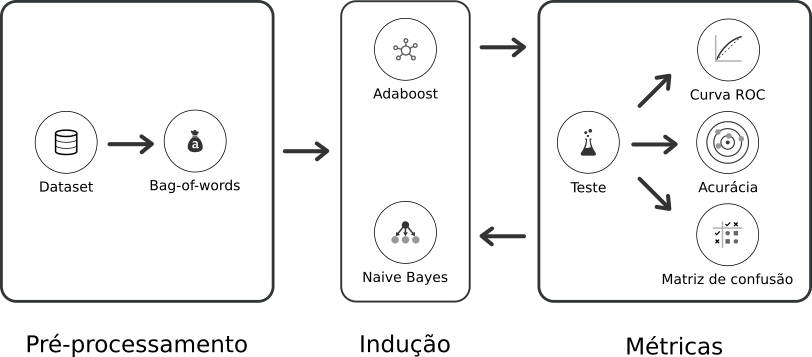
\includegraphics[scale=0.60]{images/metodologia_2.png}
\end{center}
\caption{O \textit{dataset} desbalanceado é submetido a técnica
\textit{undersampling} que gera um \textit{dataset} menor e balanceado.}
\label{figure:metodologia_2}
\end{figure}

% \newpage
\subsection{Pré-processamento, inferência indutiva e métricas de desempenho}
\label{subsection:pre_processamento}

A figura \ref{figure:metodologia_3}, ilustra as etapas necessárias para 
pré-processamento, indução e testes dos algoritmos classificadores. Devido à 
natureza textual não estruturada dos textos contidos no \textit{dataset}, no 
primeiro passo, os documentos armazenados necessitam de um pré-processamento. 
Cada sentença do texto é separada em \textit{tokens}, para transformar esses 
dados não estruturados em um formato estruturado, especificamente, uma tabela 
atributo-valor, denominada \textit{bag-of-words}. Nesta abordagem, palavras 
pouco significativas como artigos, preposições e conjunções, que pouco 
caracterizam o texto, podem ser ignoradas com uma ou mais listas de 
\textit{stopwords}. Segundo \citeonline{matsubara2003pretext}, este passo é 
importante, visto que a representação desses textos tem uma influência 
fundamental no resultado da indução dos algoritmos de Aprendizado de Máquina. 
No segundo passo, é necessário definir os parâmetros da inferência indutiva de 
cada algoritmo e induzir os modelos classificadores \textit{Adaboost} e 
\textit{Naive Bayes}. O terceiro e último passo, o resultado da inferência dos 
classificadores são avaliados com as principais métricas de análise de 
classificadores citadas na literatura de Aprendizado de Máquina. Os passos dois 
e três são repetidos até que um dos classificadores apresente resultados 
relevantes ao estudo.

\begin{figure}[H]
\begin{center}
    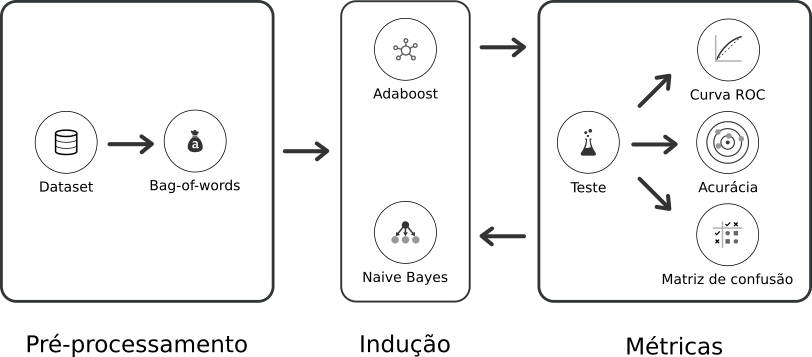
\includegraphics[scale=0.60]{images/metodologia_3.png}
\end{center}
\caption{O \textit{dataset} balanceado é submetido a técnica 
\textit{bag-of-words} no pré-processamento, resultando em uma estrutura de 
atributo-valor utilizada na inferência indutiva do classificadores, por fim, os 
modelos induzidos são avaliados por métricas de desempenho.}
\label{figure:metodologia_3}
\end{figure}

% \newpage
\subsection{Validação cruzada}
\label{subsection:validacao_cruzada}

Para avaliar e validar a hipótese proposta, foi adotada a metodologia de 
validação cruzada. O estudo de \citeonline{tavares2007estudo}, explica que esta 
abordagem consiste em fracionar o \textit{dataset} em \textbf{N} partes 
(\textit{folds}). Destas, \textbf{N}-1 partes são aplicadas na inferência 
indutiva e uma amostra é utilizada como base de testes. O método é repetido 
\textbf{N} vezes, de forma que cada fração seja utilizada apenas uma vez como 
conjunto de testes. Por fim, o resultado final é calculado pela média dos 
resultados atingidos em cada ciclo, obtendo-se assim uma estimativa da 
qualidade da inferência induzida, o que permite análises estatísticas. A Figura 
\ref{figure:metodologia_4} ilustra o fracionamento do \textit{dataset} em 
\textbf{N} partes, da qual, uma amostra é separada para testes e as demais para 
inferência indutiva, ao fim, é calculada a média dos resultados obtidos de cada 
métrica de desempenho. 

\begin{figure}[H]
\begin{center}
    
\includegraphics[scale=0.50]{images/metodologia_4.png}
\end{center}
\caption{O \textit{dataset} balanceado é fracionados en N partes, sendo uma 
parte separada para testes e as demais utilizada na indução dos classificadores, 
por fim, é calculada a média dos resultados obtidos.}
\label{figure:metodologia_4}
\end{figure}
\section{Resultados}

Este tópico é dedicado a apresentar os resultados, adversidades e contribuições 
alcançadas durante o desenvolvimento do estudo referente ao problema proposto. 
Por fim, são apresentadas considerações sobre as limitações ocorridas no 
desenvolvimento deste trabalho.

\subsection{Configuração do experimento}

Dada a matriz de referência \cite{matriz_referencia_redacao:2016}, a 
competência II foi selecionada aleatóriamente como o alvo da inferência 
indutiva dos classificadores. 

Para avaliar e validar a hipótese proposta, foram gerados resultados sobre dois 
\textit{datasets} extraidos de fontes diferentes, respectivamente (A, B).
Dentre as inúmeras possibilidades, não houve variação dos parâmetros de 
inferência indutiva dos classificadores, a fim, validar a hipótese de recuperar 
um padrão na valoração de uma redação, isto é, um dos classificadores, 
conjuntamente o mesmo, deve apresentar métricas de desempenho relevantes em 
ambos os \textit{datasets}.

\subsection{\textit{Datasets} \textbf{A} e \textbf{B}}

No caso dos \textit{datasets}, ambos dispõe da mesma quantidade de redações, com 
temas diversificados e passaram por um processo de avaliação manual com 
diferentes avaliadores. O \textit{dataset} \textbf{A} é constituído de 250 
redações, igual ao \textbf{B}. Os gráficos 
\ref{graphic:class_dataset_balanced_a} e \ref{graphic:class_dataset_balanced_b} 
demonstram a disposição das classes distintas (0.00, 0.50, 1.00, 1.50, 2.00) 
sobre a competência II, respectivamente de (\textbf{A}, \textbf{B}).

\pgfplotstableread[row sep=\\,col sep=&]{
    class & score  \\
    0.00  & 50 \\
    0.50  & 50 \\
    1.00  & 50 \\
    1.50  & 50 \\
    2.00  & 50  \\
    }\datasetAall

\begin{figure}[H]
\begin{center}
\begin{tikzpicture}
    \begin{axis}[
            ybar,
            width=8cm,
            height=7cm,
            symbolic x coords={0.00,0.50,1.00,1.50,2.00},
            bar width=10pt,
            ylabel=Quantidade,
            xlabel=Classes,
            xtick=data,
            axis lines*=left,
        ]
        \addplot[draw=black, fill=white] table[x=class,y=score]{\datasetAall};
        \node [above] at (axis cs:  0.00,50) {50};
        \node [above] at (axis cs:  0.50,50) {50};
        \node [above] at (axis cs:  1.00,50) {50};
        \node [above] at (axis cs:  1.50,50) {50};
        \node [above] at (axis cs:  2.00,50) {50};
    \end{axis}
\end{tikzpicture}
\caption{Distribuição das classes sobre a competência II de 250 redações do 
\textit{dataset} \textbf{A}.}
\label{graphic:class_dataset_balanced_a}
\end{center}
\end{figure}

\pgfplotstableread[row sep=\\,col sep=&]{
    class & score  \\
    0.00  & 50 \\
    0.50  & 50 \\
    1.00  & 50 \\
    1.50  & 50 \\
    2.00  & 50  \\
    }\datasetBall

\begin{figure}[H]
\begin{center}
\begin{tikzpicture}
    \begin{axis}[
            ybar,
            width=8cm,
            height=7cm,
            symbolic x coords={0.00,0.50,1.00,1.50,2.00},
            bar width=10pt,
            ylabel=Quantidade,
            xlabel=Classes,
            xtick=data,
            axis lines*=left,
        ]
        \addplot[draw=black, fill=white] table[x=class,y=score]{\datasetBall};
        \node [above] at (axis cs:  0.00,50) {50};
        \node [above] at (axis cs:  0.50,50) {50};
        \node [above] at (axis cs:  1.00,50) {50};
        \node [above] at (axis cs:  1.50,50) {50};
        \node [above] at (axis cs:  2.00,50) {50};
    \end{axis}
\end{tikzpicture}
\caption{Distribuição das classes sobre a competência II de 250 redações do 
\textit{dataset} \textbf{B}}
\label{graphic:class_dataset_balanced_b}
\end{center}
\end{figure}

Cada \textit{dataset} utilizado na indução foi fracionado em duas partes, esta 
divisão foi feita pela ferramenta \textit{Orange} com sucessivas reordenações 
aleatórias, de forma a garantir que ambas a partes tenham uma relação 
aproximadamente igual de exemplos positivos e negativos.

\subsection{Inferência indutiva}

No fluxo de trabalho (\textit{workflow}) da ferramenta \textit{Orange} a 
indução dos classificadores normalmente ocorre de forma automática. A aplicação
monitora o domínio do problema desenvolvido em seu \textit{workflow}, detecta 
alterações e dispara o gatilho que induz os classificadores automáticamente. 
Isso permiter facilmente realizar alterações e interpretar os resultados da 
inferência indutiva dos classificadores \cite{orange_doc}. 

\subsection{Resultados das metricas de desempenho}
% É apresentado os resultados 
% da inferência indutiva dos classificadores sobre cada \textit{dataset} a fim de
% validar a hipótese de recuperação de padrões na valoração textual.

Nos resultados do problema proposto, este estudo utilizou as principais métricas 
da literatura para análise de desempenho dos classificadores, tendo como foco 
as métricas: \textit{Acurácia} Curva ROC, e Matriz de Confusão.

A tabela ~\ref{table:evaluation_result_a} apresenta os resultados de 
\textit{acurácia} e curva ROC de cada classe do domínio, bem como, a média 
geral de cada métrica relativa a inferência indutiva dos classificadores 
\textit{Adabost} e \textit{Naive Bayes}, induzidos sobre o \textit{dataset} 
\textbf{A}.

\begin{table}[H]
\centering
\begin{tabular}{r|c|c|c|c|}
\cline{2-5}
\multicolumn{1}{c|}{}                  & \multicolumn{4}{c|}{\textbf{Dataset A}}                                            \\ \cline{2-5} 
\multicolumn{1}{l|}{}                  & \multicolumn{2}{c|}{\textbf{Adaboost}} & \multicolumn{2}{c|}{\textbf{Naive Bayes}} \\ \hline
\multicolumn{1}{|c|}{\textbf{Classes}} & \textbf{Acurácia} & \textbf{Curva ROC} & \textbf{Acurácia}   & \textbf{Curva ROC}  \\ \hline
\multicolumn{1}{|r|}{\textbf{0.00}}    & 0.627             & 0.417              & 0.787               & 0.744                \\ \hline
\multicolumn{1}{|r|}{\textbf{0.50}}    & 0.640             & 0.546              & 0.360               & 0.496                \\ \hline
\multicolumn{1}{|r|}{\textbf{1.00}}    & 0.640             & 0.381              & 0.840               & 0.339               \\ \hline
\multicolumn{1}{|r|}{\textbf{1.50}}    & 0.653             & 0.449              & 0.720               & 0.634               \\ \hline
\multicolumn{1}{|r|}{\textbf{2.00}}    & 0.787             & 0.639              & 0.907               & 0.766               \\ \hline
\multicolumn{1}{|r|}{\textbf{Média}}   & 0.669             & 0.486              & 0.722               & 0.596               \\ \hline
\end{tabular}
\caption{My caption}
\label{table:evaluation_result_a}
\end{table}

\begin{table}[H]
\centering
\begin{tabular}{cc|c|c|c|c|c|c|}
\cline{3-8}
 &  & \multicolumn{6}{c|}{\textbf{Adaboost}} \\ \cline{3-8} 
 &  & \textbf{0.00} & \textbf{0.50} & \textbf{1.00} & \textbf{1.50} & \textbf{2.00} & $\sum_{}$  \\ \hline
\multicolumn{1}{|c|}{} & \textbf{0.00} & 4 & 18 & 13 & 2 & 0 & \textbf{37} \\ \cline{2-8} 
\multicolumn{1}{|c|}{} & \textbf{0.50} & 13 & 42 & 44 & 14 & 1 & \textbf{114} \\ \cline{2-8} 
\multicolumn{1}{|c|}{} & \textbf{1.00} & 18 & 51 & 78 & 32 & 11 & \textbf{190} \\ \cline{2-8} 
\multicolumn{1}{|c|}{} & \textbf{1.50} & 7 & 14 & 31 & 15 & 2 & \textbf{69} \\ \cline{2-8} 
\multicolumn{1}{|c|}{} & \textbf{2.00} & 4 & 2 & 14 & 3 & 3 & \textbf{26} \\ \cline{2-8} 
\multicolumn{1}{|c|}{\multirow{-6}{*}{\rot{Atual}}} & $\sum_{}$ & \textbf{46} & \textbf{127} & \textbf{180} & \textbf{66} & \textbf{17} & \textbf{436} \\ \hline
\end{tabular}
\caption{Tabela de contingência ou Matriz de confusão resultante da indução do classificador AdaBoost.}
\label{tab:matrix_adaboost_a}
\end{table}

\begin{table}[H]
\centering
\begin{tabular}{cc|c|c|c|c|c|c|}
\cline{3-8}
 &  & \multicolumn{6}{c|}{\textbf{Naive Bayes}} \\ \cline{3-8} 
 &  & \textbf{0.00} & \textbf{0.50} & \textbf{1.00} & \textbf{1.50} & \textbf{2.00} & $\sum_{}$  \\ \hline
\multicolumn{1}{|c|}{} & \textbf{0.00} & 4 & 18 & 13 & 2 & 0 & \textbf{37} \\ \cline{2-8} 
\multicolumn{1}{|c|}{} & \textbf{0.50} & 13 & 42 & 44 & 14 & 1 & \textbf{114} \\ \cline{2-8} 
\multicolumn{1}{|c|}{} & \textbf{1.00} & 18 & 51 & 78 & 32 & 11 & \textbf{190} \\ \cline{2-8} 
\multicolumn{1}{|c|}{} & \textbf{1.50} & 7 & 14 & 31 & 15 & 2 & \textbf{69} \\ \cline{2-8} 
\multicolumn{1}{|c|}{} & \textbf{2.00} & 4 & 2 & 14 & 3 & 3 & \textbf{26} \\ \cline{2-8} 
\multicolumn{1}{|c|}{\multirow{-6}{*}{\rot{Atual}}} & $\sum_{}$ & \textbf{46} & \textbf{127} & \textbf{180} & \textbf{66} & \textbf{17} & \textbf{436} \\ \hline
\end{tabular}
\caption{Tabela de contingência ou Matriz de confusão resultante da indução do classificador AdaBoost.}
\label{tab:matrix_naive_a}
\end{table}

\begin{table}[H]
\centering
\begin{tabular}{r|c|c|c|c|}
\cline{2-5}
\multicolumn{1}{c|}{}                  & \multicolumn{4}{c|}{\textbf{Dataset A}}                                            \\ \cline{2-5} 
\multicolumn{1}{l|}{}                  & \multicolumn{2}{c|}{\textbf{Adaboost}} & \multicolumn{2}{c|}{\textbf{Naive Bayes}} \\ \hline
\multicolumn{1}{|c|}{\textbf{Classes}} & \textbf{Acurácia} & \textbf{Curva ROC} & \textbf{Acurácia}   & \textbf{Curva ROC}  \\ \hline
\multicolumn{1}{|r|}{\textbf{0.00}}    & 1                 & 2                  & 3                   & 4                   \\ \hline
\multicolumn{1}{|r|}{\textbf{0.50}}    & 5                 & 6                  & 7                   & 8                   \\ \hline
\multicolumn{1}{|r|}{\textbf{1.00}}    & 9                 & 10                 & 11                  & 12                  \\ \hline
\multicolumn{1}{|r|}{\textbf{1.50}}    & 13                & 14                 & 15                  & 16                  \\ \hline
\multicolumn{1}{|r|}{\textbf{2.00}}    & 17                & 18                 & 19                  & 20                  \\ \hline
\multicolumn{1}{|r|}{\textbf{Média}}   & 21                & 22                 & 23                  & 24                  \\ \hline
\end{tabular}
\caption{My caption}
\label{table:evaluation_result_b}
\end{table}


\begin{table}[H]
\centering
\begin{tabular}{cc|c|c|c|c|c|c|}
\cline{3-8}
 &  & \multicolumn{6}{c|}{\textbf{Predição}} \\ \cline{3-8} 
 &  & \textbf{0.00} & \textbf{0.50} & \textbf{1.00} & \textbf{1.50} & \textbf{2.00} & $\sum_{}$  \\ \hline
\multicolumn{1}{|c|}{} & \textbf{0.00} & 4 & 18 & 13 & 2 & 0 & \textbf{37} \\ \cline{2-8} 
\multicolumn{1}{|c|}{} & \textbf{0.50} & 13 & 42 & 44 & 14 & 1 & \textbf{114} \\ \cline{2-8} 
\multicolumn{1}{|c|}{} & \textbf{1.00} & 18 & 51 & 78 & 32 & 11 & \textbf{190} \\ \cline{2-8} 
\multicolumn{1}{|c|}{} & \textbf{1.50} & 7 & 14 & 31 & 15 & 2 & \textbf{69} \\ \cline{2-8} 
\multicolumn{1}{|c|}{} & \textbf{2.00} & 4 & 2 & 14 & 3 & 3 & \textbf{26} \\ \cline{2-8} 
\multicolumn{1}{|c|}{\multirow{-6}{*}{\rot{Atual}}} & $\sum_{}$ & \textbf{46} & \textbf{127} & \textbf{180} & \textbf{66} & \textbf{17} & \textbf{436} \\ \hline
\end{tabular}
\caption{Tabela de contingência ou Matriz de confusão resultante da indução do classificador AdaBoost.}
\label{tab:matrix_adaboost_b}
\end{table}

\begin{table}[H]
\centering
\begin{tabular}{cc|c|c|c|c|c|c|}
\cline{3-8}
 &  & \multicolumn{6}{c|}{\textbf{Predição}} \\ \cline{3-8} 
 &  & \textbf{0.00} & \textbf{0.50} & \textbf{1.00} & \textbf{1.50} & \textbf{2.00} & $\sum_{}$  \\ \hline
\multicolumn{1}{|c|}{} & \textbf{0.00} & 4 & 18 & 13 & 2 & 0 & \textbf{37} \\ \cline{2-8} 
\multicolumn{1}{|c|}{} & \textbf{0.50} & 13 & 42 & 44 & 14 & 1 & \textbf{114} \\ \cline{2-8} 
\multicolumn{1}{|c|}{} & \textbf{1.00} & 18 & 51 & 78 & 32 & 11 & \textbf{190} \\ \cline{2-8} 
\multicolumn{1}{|c|}{} & \textbf{1.50} & 7 & 14 & 31 & 15 & 2 & \textbf{69} \\ \cline{2-8} 
\multicolumn{1}{|c|}{} & \textbf{2.00} & 4 & 2 & 14 & 3 & 3 & \textbf{26} \\ \cline{2-8} 
\multicolumn{1}{|c|}{\multirow{-6}{*}{\rot{Atual}}} & $\sum_{}$ & \textbf{46} & \textbf{127} & \textbf{180} & \textbf{66} & \textbf{17} & \textbf{436} \\ \hline
\end{tabular}
\caption{Tabela de contingência ou Matriz de confusão resultante da indução do classificador AdaBoost.}
\label{tab:matrix_naive_b}
\end{table}



% \begin{table}[H]
% \centering
% \begin{tabular}{c|c|c|c|c|c|}
% \cline{2-6}
%  & \multicolumn{5}{c|}{\textbf{Resultado da avaliação}} \\ \hline
% \multicolumn{1}{|c|}{\textbf{Classes}} & \textbf{ROC} & \textbf{Acurácia} & \textit{\textbf{F-Score}} & \textit{\textbf{Precision}} & \textit{\textbf{Recall}} \\ \hline
% \multicolumn{1}{|c|}{\textbf{0.00}}  & 0.498 & 0.828 & 0.096 & 0.845 & 0.828 \\ \hline
% \multicolumn{1}{|c|}{\textbf{0.50}}  & 0.552 & 0.640 & 0.349 & 0.653 & 0.640 \\ \hline
% \multicolumn{1}{|c|}{\textbf{1.00}}  & 0.499 & 0.509 & 0.422 & 0.506 & 0.509 \\ \hline
% \multicolumn{1}{|c|}{\textbf{1.50}}  & 0.549 & 0.579 & 0.222 & 0.755 & 0.759 \\ \hline
% \multicolumn{1}{|c|}{\textbf{2.00}}  & 0.541 & 0.915 & 0.140 & 0.899 & 0.915 \\ \hline
% \multicolumn{1}{|c|}{\textbf{Média}} & \textbf{0.529} & \textbf{0.694} & \textbf{0.246} & \textbf{0.737} & \textbf{0.730} \\ \hline
% \end{tabular}
% \caption{Resultado das métricas de desempenho do classificador AdaBoost.}
% \label{tab:evaluation_result}
% \end{table}

% A adversidade de classes desbalanceadas, pode produzir um modelo com elevadas taxas de acurácia global para determinadas classes, como o ocorrido nas classes 0.00 e 2.00 de 0.828 e 0.915 respectivamente, entretanto frequentemente tende a prejudicar a identificação de exemplos pertencentes a grupos minoritários.

% Ilustrada na Figura ~\ref{fig:roc}, a representação gráfica da Curva ROC de cada classe induzida pelo classificador.

% \begin{figure}[H]
% \begin{center}
%     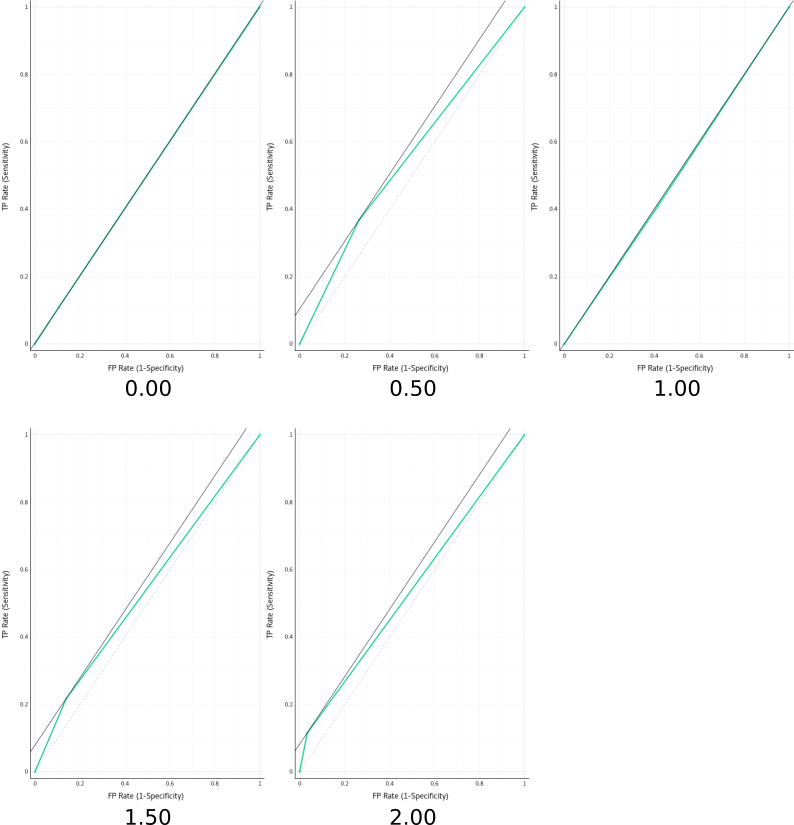
\includegraphics[scale=0.75]{images/roc.png}
% \end{center}
% \caption{Representação gráfica da Curva ROC para cada classe (0.00, 0.50, 1.00, 1.50 e 2.00) induzida no modelo AdaBoost.}
% \label{fig:roc}
% \end{figure}

% O comportamento esperado para a curva, é que a mesma, se aproxime o máximo possível de 1 em cada classe. Entretanto a métrica se apresenta como uma reta nas classes 0.00 e 1.00, nas demais classes tende sutilmente a 1. Conclui-se que a predição das classes 0.00 e 1.00 nos testes estão ocorrendo de forma aleatório pelo classificador.

% Por fim a tabela de contingência ou matriz de confusão, que através da discriminação dos erros ou acertos preditos para cada classe demonstra o desempenho do classificador, uma das métricas mais eficiente de se analisar um classificador. 

% A Tabela ~\ref{tab:matrix_confusion} exibe ao longo da diagonal em tons de cinza as decisões corretas: número de verdadeiros positivos TP e verdadeiros negativos TN; já os elementos fora dessa diagonal representam os erros cometidos: número de falsos positivos FP e falsos negativos FN. É notável que o valor ideal fora da diagonal seja sempre igual a 0.  

% \begin{table}[H]
% \centering
% \begin{tabular}{cc|c|c|c|c|c|c|}
% \cline{3-8}
%  &  & \multicolumn{6}{c|}{\textbf{Predição}} \\ \cline{3-8} 
%  &  & \textbf{0.00} & \textbf{0.50} & \textbf{1.00} & \textbf{1.50} & \textbf{2.00} & $\sum_{}$  \\ \hline
% \multicolumn{1}{|c|}{} & \textbf{0.00} & 4 & 18 & 13 & 2 & 0 & \textbf{37} \\ \cline{2-8} 
% \multicolumn{1}{|c|}{} & \textbf{0.50} & 13 & 42 & 44 & 14 & 1 & \textbf{114} \\ \cline{2-8} 
% \multicolumn{1}{|c|}{} & \textbf{1.00} & 18 & 51 & 78 & 32 & 11 & \textbf{190} \\ \cline{2-8} 
% \multicolumn{1}{|c|}{} & \textbf{1.50} & 7 & 14 & 31 & 15 & 2 & \textbf{69} \\ \cline{2-8} 
% \multicolumn{1}{|c|}{} & \textbf{2.00} & 4 & 2 & 14 & 3 & 3 & \textbf{26} \\ \cline{2-8} 
% \multicolumn{1}{|c|}{\multirow{-6}{*}{\rot{Atual}}} & $\sum_{}$ & \textbf{46} & \textbf{127} & \textbf{180} & \textbf{66} & \textbf{17} & \textbf{436} \\ \hline
% \end{tabular}
% \caption{Tabela de contingência ou Matriz de confusão resultante da indução do classificador AdaBoost.}
% \label{tab:matrix_confusion}
% \end{table}

% \subsection{Considerações Finais}

% E notável que adversidade de classes desbalanceadas influenciou consideravelmente nos resultados preliminares.  A próxima etapa deste estudo merece destaque em uma seção exclusiva para discussão do tema e a análise dos principais métodos na literatura para balanceamento de classes.

% As dificuldades observadas no estudo do problema proposto motivam melhorias e o surgimento de novas estratégias pra a continuidade do trabalho. 

% Os primeiros experimentos realizados na predição, ilustrado no Gráfico abaixo, demonstraram uma taxa de 30\% de acerto na predição da primeira competência exigida em um texto de redação, de uma amostra de 100 redações. 

% A análise gráfica do resultado experimental demonstra que a predição do modelo está em uma faixa especifica de 0.5 a 1.5, ou seja, a indução do modelo deve ser repetida até o mesmo se tornar genérico.

% \pgfplotstableread[col sep=semicolon]{data/adaboost_competence_1.dat}\data
% \begin{figure}[H]
% \begin{center}

% \begin{tikzpicture}
%     \begin{axis}[
%         title=Demonstrar domínio da norma padrão da língua escrita. (1ªCompetência ),
%         width=\textwidth,
%         ymin=0,
%         ytick={0,0.5,1.0,1.5,2.0},
%         ylabel=Pontuação,
%         xtick=data,
%         xticklabel style={rotate=90,anchor=east},
%         xticklabels from table={\data}{title},
%         legend style={ legend columns=-1},
%         enlarge x limits=0.01
%         ]
%         \addplot table[x=id, y=comp1] {\data};
%         \addplot table[x=id, y=adaboost] {\data};
%         \legend{Profissional,AdaBoost}
%     \end{axis}
% \end{tikzpicture}
% \end{center}
% \end{figure}


% \section{Discussão}

Na \autoref{subsection:pre_processamento} e explicado o uso da abordagem
\textit{bag-of-words}, apesar de inumeráveis configurações possíveis sobre este 
método, o mesmo foi utilizado em sua forma canônica, por fim, o objetivo era de 
não interfirir na assinatura do padrão encontrado no texto.

Conforme foi explicado na \autoref{subsection:validacao_cruzada} na validação 
cruzada, o \textit{dataset} balanceado foi dividido em dez partes iguais. Em 
testes anteriores foi observado, que devido a um número limitado de textos no 
\textit{dataset}, a quantidade superior as dez partições não influenciava 
diretamente os resultados das métricas de desempenho, entretanto, onerava 
consideravelmente o tempo de inferência indutiva dos classificadores.


\section{Conclusão}

Este trabalho teve por objetivo o estudo da recuperação de padrões na valoração 
textual de redações, através da classificação de textos. Destaca-se que foram 
realizadas extensas avaliações empíricas sobre os classificadores 
\textit{Naive Bayes} e \textit{Adaboost}, no decorrer das atividades 
desenvolvidas para atingir os objetivos propostos, no entanto, por ser um campo 
de estudo relativamente recente e em contínuo desenvolvimento, acredito que 
ainda exista um grande espaço para novas descobertas.

Como contribuição, este trabalho demonstra que é possível se beneficiar com os 
padrões recuperados em textos. A recuperação de padrões implícitos em textos 
abre precedente a explorar novas soluções na valoração automática dos textos 
de redação.
\section{Trabalhos Futuros}

Para trabalhos futuros pretende-se estudar e aperfeiçoar as técnicas de 
pré-processamento e extração de atributos com o objetivo de mensurar com maior 
representatividade o padrão encontrado dentro do texto, obtendo uma melhor 
separação entre as valorações de competências.
\section{Considerações finais}

Na \autoref{subsection:pre_processamento}, é explicado o uso da abordagem
\textit{bag-of-words}, apesar de inumeráveis configurações possíveis sobre este 
método, o mesmo foi utilizado em sua forma canônica, por fim, o objetivo era de 
não interfirir na assinatura do padrão encontrado no texto.

Conforme foi definido na \autoref{subsection:configuracao}, na utilização da 
validação cruzada, o \textit{dataset} foi dividido em dez partes iguais. Em 
testes anteriores foi observado, que a quantidade superior as dez partições 
não influenciava diretamente os resultados das métricas de desempenho, 
entretanto, onerava consideravelmente o tempo de inferência indutiva dos 
classificadores.

A quantidade de exemplos da competência III obtida no \textit{dataset} na 
\autoref{subsection:balanceamento}, pode apresentar-se de uma certa forma 
modesta, entretanto, normalmente é suficientemente para produzir resultados 
relevantes.
    

\bibliography{references}

\end{document}
